\documentclass[a4paper,12pt]{report}
\addtolength{\oddsidemargin}{-1.cm}
\addtolength{\textwidth}{2cm}
\addtolength{\topmargin}{-2cm}
\addtolength{\textheight}{3.5cm}
\newcommand{\HRule}{\rule{\linewidth}{0.5mm}}
\makeindex

\usepackage{longtable}
\usepackage{graphicx}
\usepackage{makeidx}
\usepackage{hyperref}
\usepackage{verbatim}

\hypersetup{
    colorlinks=true,
    linkcolor=blue,
    filecolor=magenta,      
    urlcolor=cyan,
}


% define the title
\author{Team Lima}
\title{ Assignment 1}
\begin{document}
\setlength{\parskip}{6pt}

% generates the title
\begin{titlepage}

\begin{center}
% Upper part of the page       

\includegraphics[width=1\textwidth]{./images/up-logo.jpg}\\[0.4cm]    
\textsc{\LARGE Department of Computer Science}\\[1.5cm]
\textsc{\Large COS 301 - Mini Project}\\[0.5cm]
% Title
\HRule \\[0.4cm]
{ \huge \bfseries Assignment 1}\\[0.4cm]
\HRule \\[0.4cm]
% Author and supervisor
\begin{minipage}{0.4\textwidth}
\begin{flushleft} \large
\emph{Author:}\\
Tshepo {Malesela}
\end{flushleft}
\end{minipage}
\begin{minipage}{0.4\textwidth}
\begin{flushright} \large
\emph{Student number:} \\
u14211582
\end{flushright}
\end{minipage}
\begin{minipage}{0.4\textwidth}
\begin{flushleft} \large
\emph{} \\
Kevin David {Heritage}
\end{flushleft}
\end{minipage}
\begin{minipage}{0.4\textwidth}
\begin{flushright} \large
\emph{} \\
u13044924
\end{flushright}
\end{minipage}
\begin{minipage}{0.4\textwidth}
\begin{flushleft} \large
Unarine {Rambani}
\end{flushleft}
\end{minipage}
\begin{minipage}{0.4\textwidth}
\begin{flushright} \large
\emph{} \\
u14004489
\end{flushright}
\end{minipage}
\begin{minipage}{0.4\textwidth}
\begin{flushleft} \large
Vukile {Langa}
\end{flushleft}
\end{minipage}
\begin{minipage}{0.4\textwidth}
\begin{flushright} \large
\emph{} \\
u14035449 
\end{flushright}
\end{minipage}
\begin{minipage}{0.4\textwidth}
\begin{flushleft} \large
Wynand Hugo Meiring
\end{flushleft}
\end{minipage}
\begin{minipage}{0.4\textwidth}
\begin{flushright} \large
\emph{} \\
u13230795  
\end{flushright}
\end{minipage}
\begin{minipage}{0.4\textwidth}
\begin{flushleft} \large
Nontokozo Hlastwayo
\end{flushleft}
\end{minipage}
\begin{minipage}{0.4\textwidth}
\begin{flushright} \large
\emph{} \\
u14414555
\end{flushright}
\end{minipage}
\begin{minipage}{0.4\textwidth}
\begin{flushleft} \large
Tim Kirker
\end{flushleft}
\end{minipage}
\begin{minipage}{0.4\textwidth}
\begin{flushright} \large
\emph{} \\
u11152402
\end{flushright}
\end{minipage}
\vfill

{\large \today}
\end{center}
\end{titlepage}
\footnotesize
\normalsize

\renewcommand{\thesection}{\arabic{section}}
\newpage
\begin{center}
\textsc{\LARGE Requirements Specification}\\[1.5cm]
\textsc{\Large Team Lima github repository link}\\[0.5cm]
For further references see \href{https://https://github.com/slugger7/team-lima}{gitHub}.
\today
\end{center}


\newpage
\section{Introduction}
In this section we will explore an overview of everything that is included in the Software Requirements Specification (SRS) document.

\subsection{Purpose}
The purpose of this document is to give a detailed description of the features of the Mini-Project, to serve as a guide or reference for the software developers and primarily a proposal to the client approval.

\subsection{Scope}
The Mini-Project(Publication System) is a web and Android application which will assist research leaders as well as the heads of department to keep track of the progress of different research groups.
\newline Users(UP Staff) will act as the administrators for the different research groups and provide information regarding research topics, group members, progress, etc using the web-portal.
\newline The system will only keep track of metadata and not contain any of the actual publications. The information is maintained in a database that is located on a web-server. An internet connection will be required to fetch and display the information.

\subsection{Overview}

The remainder of this document includes four more sections and is organized as follows:
\newline Section 2 describes the Vision, which basically explains what the client wants to achieve with the project and what the average user would get out of the product.Section 3 continues to discuss the background, which includes the business/ research opportunity to simplify the administration and management of documents/publications in the world of research. This section also sheds light on the problems being faced that may have led to this project being started. Section 4 presents the Architecture requirements to the reader, including the integration and quality requirements as well as the architectural constraints. Section 5 describes the Functional Requirements and captures all the functionality which would be required by the users of the system. Section 6 brings up the Open Issues which entail anything that needs to be clarified regarding the requirements as well as any irregularities/inconsistencies found in the requirements.


\newpage
\section{Vision}
\subsection{Product Functions}
The main aim of this system is to assist researchers(authors) and head of department with storing metadata of research papers(not the paper itself). In the system the users will be able to see how many papers is that particular user working on,  identify which research papers  are due at what time(the system will keep a daily reminder of the due date) and who are the other author of the paper but will maintain privacy since a user won't be able to see other user's work(only going to see papers where the user co-author) unless it is the head of department or a supervisor.The system will keep a status of the paper(still working on it,submitted waiting for feedback,rejected, accepted,published or improving it after rejection).
\newline The system should be able support 100 users concurrently without any difficulties.The head of department is allowed to see everything in the system meaning everyone's work. An author is not necessarily a user of the system meaning that a person can be added as one of the authors of a certain research paper, while they are not a user of the system, the primary author is responsible of adding and deleting authors for a paper and the primary should be a user of the system.
\newline Every research paper on the system should have at least one user responsible for it. The system keeps the title of the paper, if a paper is accepted/published a link to where the actual paper is stored,if a paper is deleted in the system(by the primary author) a reason, should be provided for that termination, the type of a paper(journal, conference paper or book chapter) is also kept in the system, and the system should also keep report containing DoE Units, DoE Research Output Units,UPWeighted Research Outputs, Estimated DoE Outputs and Research Funding.

\subsection{User classes and characteristics}
\subsubsection{Head of Department}
	\begin{itemize}
		\item Must be a registered user of the user of the system.
		\item There is only one head of Department, since the system is for one department.
		\item Able to see everyone's work on the system.
		\item May be an author.
		\item May add or delete papers.
	\end{itemize}

\subsubsection{Primary Author/ Leading Researcher}
	\begin{itemize}
		\item Must be a registered user of the user of the system.
		\item Any number less than a hundred.
		\item Able to see only the list papers of where is authoring or co-authoring.
		\item Can add or delete papers.
		\item Can add or delete authors.
	\end{itemize}

\subsubsection{Author}
	\begin{itemize}
		\item May or may not be a user of the system.
		\item If a user able to see only the list papers of where is co-authoring.
		\item Otherwise not able to see anything in the system.
	\end{itemize}

\subsection{Operating Environment}
The system will be a standalone system, it does not load any external module or library function. For the user to login to the system, they must have internet access. When a user modifies something, every other use who has access to the information needs access to its latest version. The system must run on any operating system, and it will have make use of a virtual interface for the different operating system and hardware platforms.

\newpage
\section{Background}
The system give  different authors/researchers who are working on the same paper an opportunity to be able to stay updated about the progress of the paper. The system also gives the head of department an opportunity to better supervise the staff members on the research  they are working on,since research is one of the crucial aspects of every department in the university. The system also gives the head of department an opportunity to evaluate the staff member using the report the system provides.

A correct usage of the system will yield good results in management of the department's research activity and will also provide a better way of co-authoring among different authors/users because when there is a change in the status of the paper every author and user will be made aware of the deadline.

The system will also improve the current way of storing research metadata the department uses, which is  writing everything on a spreadsheet. The system will also add other things that are not in the spreadSheet like a full report of how the whole department is performing with regards to research papers and provide a more informed way of co-authoring, since everyone working on the paper will know what is going on.
\newpage
\section{Architecture requirements}
\subsection{Access channel requirements}

There will be multiple access channels for the proposed system. Mobile/android application clients will be used to fetch data(such as the deadline dates) and integrate them into mobile device for users to easily be able to identify when their deadlines are  for. The mobile application will also allow a user to search for and identify the type of paper(journal, conference paper or book) that is being worked on as well as how many papers a user may be working on. The mobile application will also allow users to see the status of a paper(still working on it, submitted and waiting for feedback, rejected, accepted, published or improving after rejection).
Web servers will be used in order to store all the users and their details as well as all the papers that are being worked on by any particular user. These web servers will be set up such that 100 users can concurrently access the server without any difficulties. The system will also make due with browser clients that will have all the same functionality as the mobile client and allow any user to access the system where ever they may be. Both the mobile application and browser client will interact with the web server in order to gain access to any information it might need. 


\subsection{Quality requirements}


In order to create a safe and legitimate system that will meet all the specifications of the project, some system requirements such as how the system performance, security, flexiblity, maintainability, auditablity, integrability, cost and usabilty.

\subsubsection{Performance} 

The system has to responsive, and responsive enough to handle up to one hundred users and not lag, the system must also be perform in such a way that if certain authors responsible for a paper want to access it at the same time them can without the system slowing down.

\subsubsection{Security}
The most important security measure that needs to held in this system is that only U.P staff are allowed to register as users, and may be the only member who can access the link to view papers. They will either set their own usernames or use their access card numbers in place of their usernames. They will also be required to set their own passwords. This password should be at least eight characters long to make it a bit more difficult for potential hackers to gain access.If a user forgets his/her password, there will need to be a way of retrieving it or re-setting a new one. My group and I decided that an email containing a link should be sent out to a user directing them to a page whereby they will be able to set a new password. If a user also fails to get the correct password for more than three tries, the user account should be blocked for safety reasons, and the user should be sent an email following the password re-setting procedure. If system fails to allow a user back into the system, the user needs to direct an enquiry to the administative user.
The user also is given the power to remove or add authors the a paper, they may also choose to terminate the paper and should also be given access to revive that same paper that was terminated by them. Only users involved in the publication can edit a paper, this modification must be known by the other users involved in the same paper, so some system of alerting co-users about the modification. The system will also have user profiles, a user can only edit their own profile. The system also has super-users that have more control then users, they can access all publications. There are alos administrative users and control who has access the the system.The administrative users basically can  remove or add users to the system, they also fix any problems regarding users. They can also view the activities of a particular user and because of this, all user activity must be logged. The hierarchy of this system in terms of privilege is tha tadministrative users have the most priority, super-users have the more authority than users and finally authors have the least aauthority.

\subsubsection{Reliability}

Reliability for this application to work is crucial to its success. If a user wants to access a paper and it is urgent, the user must always be able to access what they have access to at all times without the system failing fetch the information the user seeks. Reliability includes keeping track of user authority, the system cannot ever loose track of what actions each user can perform on the system. Super-users must be able to do all their administrative jobs, if that could fail then they would nit be able to keep track of user activity and the application. 

\subsubsection{Flexibility}

This application should be web-based and should also have a mobile application that users can make use of when away from a desktop or laptop. The system needs to be able to run the same on all these platforms and users must be able to do the same things on the web-based application and mobile-based application. For the mobile side of things, this application needs to be able to support older versions of android mobile system, so that no matter the device is used, a user can access the application and look up what they need at all times.

\subsubsection{Maintainability}

Maintenance of this application will be handled by the super-users. With just a little over one hundred users this system will have to be well maintained to be able to run things smoothly.

\subsubsection{Monitorability}

The super-users will be in charge of monitoring users activity. Since there will be a log for each users activity on the system, the super user can look at the log to see what a specific user has been doing. Everything in the system will be logged to increase the level of monitorability.

\subsubsection{Usability}

This application should be simple enough for a user to use without the user asking for assistance more than once. The system must have basic instruction, maybe given to the user on a basic pdf file that they can read and understand how to navigate the system. If users still do not have a clear perspective on how the system works they will just keep referring to the pdf.

\subsubsection{Cost}

The system being built should be complex enough to run smoothly on all devices but also it should be maintainable by students to cut costs and man hours.

\subsubsection{Integrability}

The system should be integrable to mobile devices and not just be web-based. There will be a mobile application for this system.


\subsection{Integration requirements}



\subsection{Architecture constraints}

The server should be available at all times to allow all users to login at any time. There should be search functionality to allow users to navigate faster.The system will be web-based and will also built to to run on mobile devices.

\subsubsection{Web-based development}

We will be building the web-based system using HTML, CSS, and some javascript for some user side functionality. We will do all client validation using javascript to check if the user input is valid.  

\subsubsection{Server-side development}

To run the database we will be using mySQL and PHP. We will store the user profile using a mySQL database and use, and all validation will be done in PHP.


\subsubsection{Mobile application development}

To build the mobile application, we will use androidStudio(java). The mobile application should only be able to access the server when you are within the premises of the University.

\newpage
\section{Functional requirements and application design}
This section discusses the application functionality required by users (and other stakeholders).
\subsection{Use case prioritization}
\subsubsection{Critical}
	\begin{itemize}
		\item The system needs to be able to handle 100 users concurrently and at the same time.
		\item Only University of Pretoria staff members may register to become users.
		\item Users are only allowed to see publications that they are involved in.
		\item There should be a a superuser or root account for the Head of Department, the superuser should be able to see all research papers that is on the system.
		\item There should be a a superuser or root account for the Head of Department, the superuser should be able to see all research projects that is on the system.
		\item Users and authors should be able to upload their documents to the research project.
	\end{itemize}

\subsubsection{Important}
	\begin{itemize}
		\item Users(UP staff) can add and remove authors.
		\item Users(UP staff) decide when the deadline of a research paper is.
		\item Users(UP staff) can terminate a research paper and revive a terminated research paper.
		\item A user can edit the details about a research paper that they are involved in.
		\item User profiles should show the total accumulated units.
		\item The system has to log everything.
		\item Users must be able to enter historical data (previously completed research papers).
		\item Every research paper only has one primary author.
		\item Users(UP staff) decide when the deadline of a research project is.
		\item Users(UP staff) can terminate a research project and revive a terminated research project.
		\item A user can edit the details about a research project that they are involved in.
		\item User profiles should show the total accumulated units.
		\item The system has to log everything.
		\item Users must be able to enter historical data (previously completed research projects).
		\item Every research project only has one primary author.
		\item Co-authors are added and sequenced.
	\end{itemize}

\subsubsection{Nice-To-Have}
\begin{itemize}
\item There should be a checkbox that defaults users as authors for research papers that they administrate, if they are just administrating they should explicitly uncheck that they are not an author.
\item There should be an indication of progress on research papers (progress bar/percentage indication of work done)
\item Users should be able to search for authors if they have been stored in the system.
	\end{itemize}


	
\subsection{Use case/Service Contracts}
\subsubsection{Critical}
	Handle 100 users concurrently
	\begin{itemize}
		\item Pre-conditions
			\begin{itemize}
				\item System needs to be online.
				\item Users need to connect to the system.
				\item System needs to have concurrency controls to help aid 100 users at the maximum.
			\end{itemize}
		\item Post-conditions
			\begin{itemize}
				\item System can successfully maintain the concurrent use of 100 users.
			\end{itemize}
	\end{itemize}

	Only UP staff members may register to become users
	\begin{itemize}
		\item Pre-conditions
			\begin{itemize}
				\item User needs to be registered at the University of Pretoria.
				\item User needs a valid staff number from the University of Pretoria.
			\end{itemize}
		\item Post-conditions
			\begin{itemize}
				\item User that is now registered on the system may now add research projects and so forth.
			\end{itemize}
	\end{itemize}

	The superuser account
	\begin{itemize}
		\item Pre-conditions
			\begin{itemize}
				\item User needs to be a staff member at the University Of Pretoria.
				\item User needs to be the head of the department.
			\end{itemize}
		\item Post-conditions
			\begin{itemize}
				\item Super user can see all research projects on the system.
				\item Super user has control of the whole system.
			\end{itemize}
	\end{itemize}

	Users and authors should be able to upload their documents to the research project
	\begin{itemize}
		\item Pre-conditions
			\begin{itemize}
				\item User should be registered on the system
				\item User should be involved on the research project they want to upload a document to.
			\end{itemize}
		\item Post-conditions
			\begin{itemize}
				\item User is able to upload a document to the research project for the rest of the users/authors to see.
			\end{itemize}
	\end{itemize}

\subsubsection{Important}
	Users can add and remove authors
	\begin{itemize}
		\item Pre-condition
			\begin{itemize}
				\item User has to be registered on the system.
				\item User has to be the primary author on a research project that they want to add and remove other authors to and from.
			\end{itemize}
		\item Post-condition
			\begin{itemize}
				\item User can add and remove authors from the research project that they are the primary author on.
			\end{itemize}
	\end{itemize}

	Users decide when the deadline of a research project is.
	\begin{itemize}
		\item Pre-conditions
			\begin{itemize}
				\item Users need to be registered on the system.
				\item Users need to be a primary author on a research project for which they want to set a deadline.
				\item Deadline cannot be in the past.
			\end{itemize}
		\item Post-conditions
			\begin{itemize}
				\item Deadline is set on the research project.
				\item All co-authors are notified via email what the deadline on that research project is.
			\end{itemize}
	\end{itemize}

	Users can terminate and revive a research project
	\begin{itemize}
		\item Pre-conditions
			\begin{itemize}
				\item User needs to be registered on the system.
				\item User needs to be the primary author on the research project which needs to be terminated or revived.
			\end{itemize}
		\item Post-conditions
			\begin{itemize}
				\item The selected research project is terminated or revived.
				\item All co-authors are notified via email that the research project is terminated or revived.
			\end{itemize}
		\item Exceptions
			\begin{itemize}
				\item Superuser also has control over any users research project.
			\end{itemize}
	\end{itemize}

	Users can edit details about a research paper they are involved in
	\begin{itemize}
		\item Pre-conditions
			\begin{itemize}
				\item User has to be registered on the system.
				\item User has to be added to the research project or be the primary author.
				\item There has to be a research paper uploaded to the system on which the details need to be changed.
			\end{itemize}
		\item Post-conditions
			\begin{itemize}
				\item The details of the research paper can be edited by the author.
				\item All co-authors can see the edited details of the research paper.
			\end{itemize}
	\end{itemize}

	User profiles should show the total accumulated units
	\begin{itemize}
		\item Pre-conditions
			\begin{itemize}
				\item User has to be registered on the system.
				\item User needs to be involved on a research project.
			\end{itemize}
		\item Post-conditions
			\begin{itemize}
				\item Users profile will show the total accumulated units of contributions.
			\end{itemize}
	\end{itemize}

	The system has to log everything
	\begin{itemize}
		\item Pre-conditions
			\begin{itemize}
				\item System has to be online.
			\end{itemize}
		\item Post-conditions
			\begin{itemize}
				\item Everything that any user does on the system is added to a log.
			\end{itemize}
	\end{itemize}

	Users must be able to enter historical data
	\begin{itemize}
		\item Pre-conditions
			\begin{itemize}
				\item User must be registered on the system.
				\item User must be involved with a research project.
				\item There must be a previously completed research paper/project on which historical data needs to be entered.
			\end{itemize}
		\item Post-conditions
			\begin{itemize}
				\item Historical data is added to the previously completed research paper/project.
				\item All co-authors can see this historical data that has been added about the previously completed research paper/project.
			\end{itemize}
	\end{itemize}

	Every research project has only one primary author
	\begin{itemize}
		\item Pre-conditions
			\begin{itemize}
				\item User needs to be registered on the system.
				\item User has to be the creator of the research project or superuser.
			\end{itemize}
		\item Post-conditions
			\begin{itemize}
				\item User becomes the primary author on the research project.
			\end{itemize}
		\item Exceptions
			\begin{itemize}
				\item User that used to be the primary author hands the research project over to one of the co-authors to become the primary author.
			\end{itemize}
	\end{itemize}

	Co-authors are added and sequenced
	\begin{itemize}
		\item Pre-conditions
			\begin{itemize}
				\item Co-authors need to be registered on the system.
				\item The primary author needs to specify which authors to add to the research project.
			\end{itemize}
		\item Post-conditions
			\begin{itemize}
				\item Co-authors are added to the research project and sequenced in a hierarchy.
			\end{itemize}
	\end{itemize}

\subsubsection{Nice-to-Have}
	Users are authors by default for research projects that they administrate. If the user is only an administrator they should explicitly mark them self as administrator only
	\begin{itemize}
		\item Pre-conditions
			\begin{itemize}
				\item User needs to be registered on the system.
				\item User needs to be an administrator of a research project or
				\item User needs to be the primary author of a research project.
			\end{itemize}
		\item Post-conditions
			\begin{itemize}
				\item User can remove themselves as an author and only be an administrator of the research project.
			\end{itemize}
		\item Exceptions
			\begin{itemize}
				\item Superuser is an administrator on all research project.
			\end{itemize}
	\end{itemize}

	Indication of progress on research projects
	\begin{itemize}
		\item Pre-conditions
			\begin{itemize}
				\item The system needs to have a research project that has active authors.
			\end{itemize}
		\item Post-conditions
			\begin{itemize}
				\item There is a progress bar of how much work is done on that research project before the research project is completed.
			\end{itemize}
	\end{itemize}

	Users should be able to search for other authors
	\begin{itemize}
		\item Pre-conditions
			\begin{itemize}
				\item User should be registered on the system
				\item Other users should be registered on the system
			\end{itemize}
		\item Post-conditions
			\begin{itemize}
				\item User has the ability to search in the system for other users/authors.
			\end{itemize}
	\end{itemize}

\newpage

\subsection{Required functionality}
\subsubsection{Critical use cases}

\begin{flushleft}
	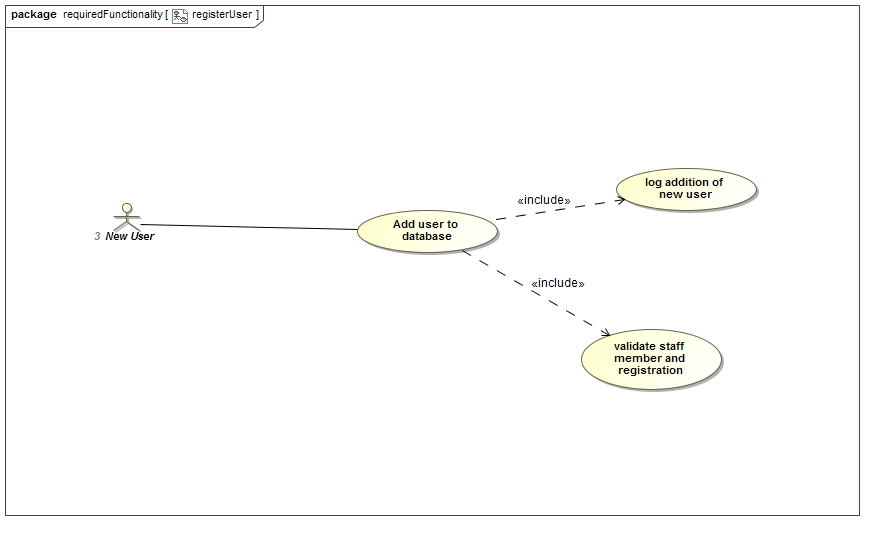
\includegraphics[scale=0.5]{./images/uc__registerUser.jpg}
	\begin{center}
		Only UP staff members may register to become users
	\end{center}

	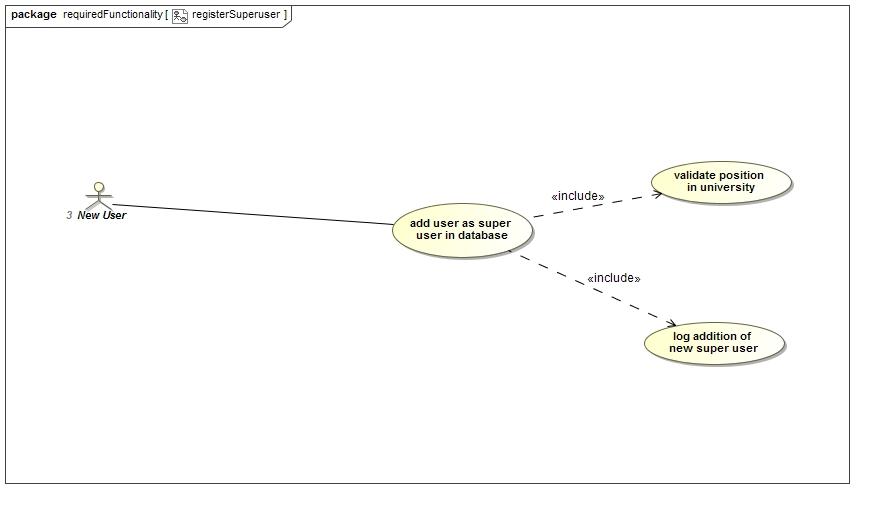
\includegraphics[scale=0.5]{./images/uc__registerSuperuser.jpg}
	\begin{center}
		Creating the super user account
	\end{center}
\end{flushleft}

\newpage

\begin{flushleft}
	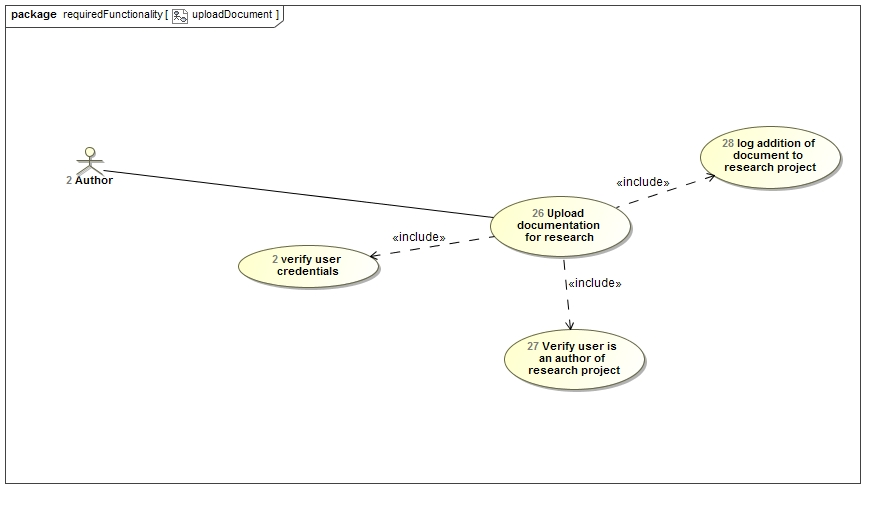
\includegraphics[scale=0.5]{./images/uc__uploadDocument.jpg}
	\begin{center}
		Users should be able to upload their documents
	\end{center}
\end{flushleft}

\newpage
\subsubsection{Important use cases}

\begin{flushleft}
	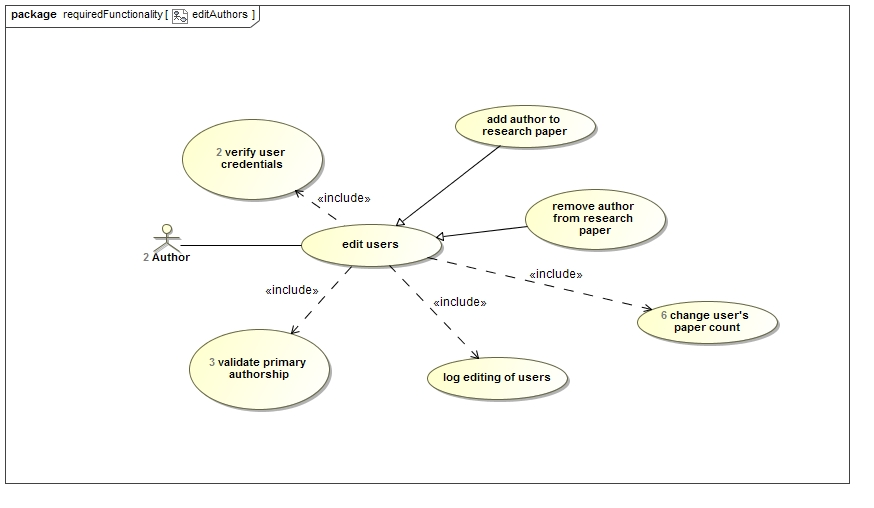
\includegraphics[scale=0.5]{./images/uc__editAuthors.jpg}
	\begin{center}
		Users can add and remove authors
	\end{center}

	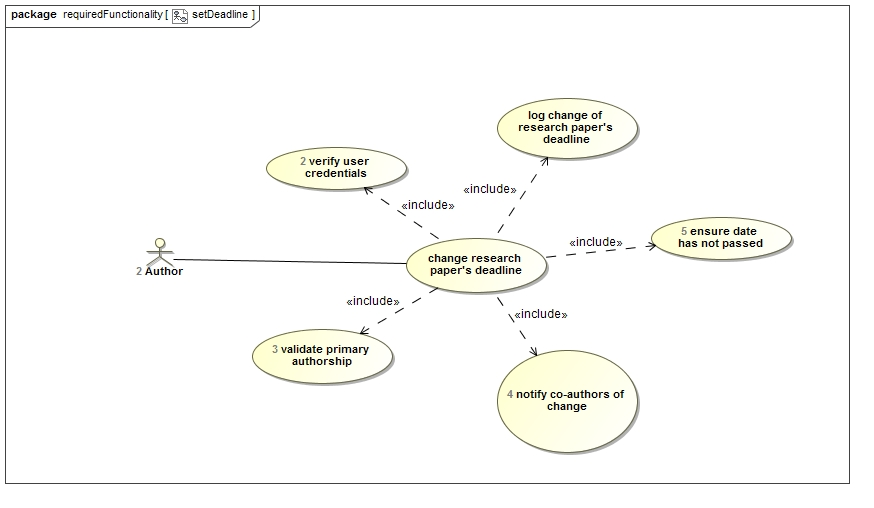
\includegraphics[scale=0.5]{./images/uc__setDeadline.jpg}
	\begin{center}
		Users decide the deadline of a research project
	\end{center}
\end{flushleft}

\newpage

\begin{flushleft}
	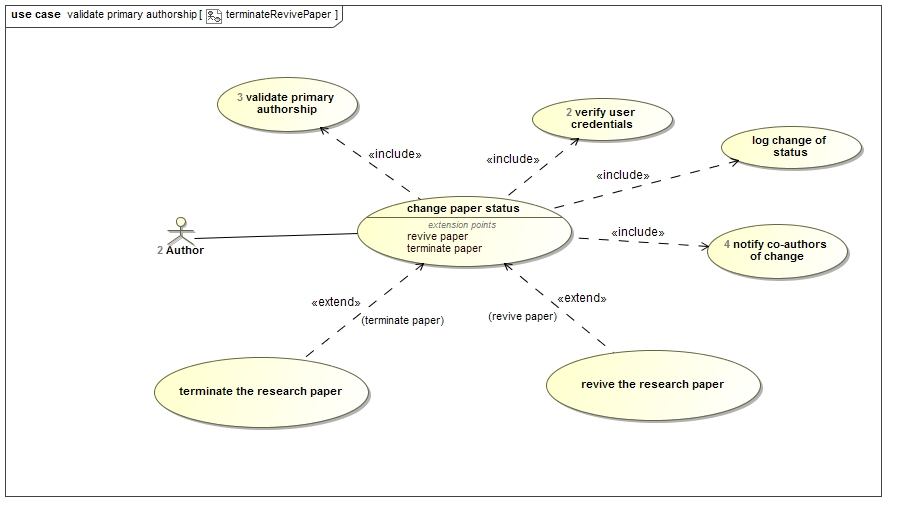
\includegraphics[scale=0.5]{./images/uc__validate_primary_authorship__terminateRevivePaper.jpg}
	\begin{center}
		Users can terminate and revive a research project
	\end{center}

	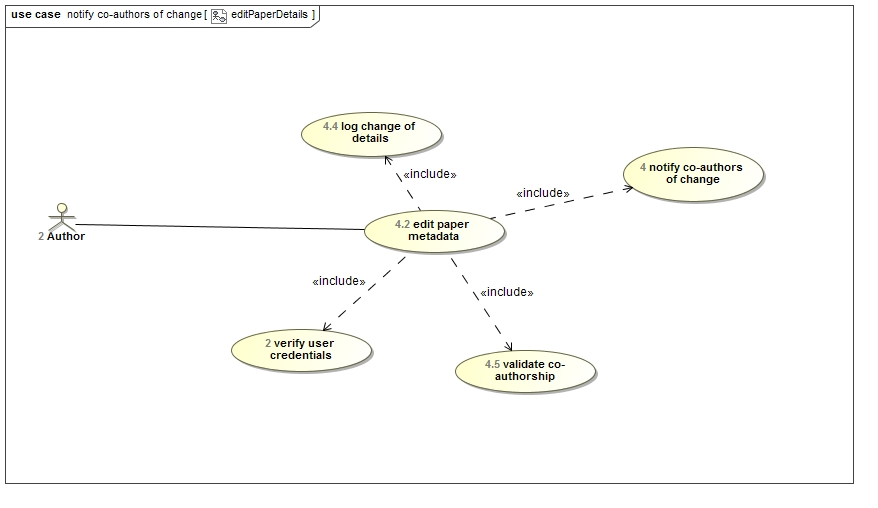
\includegraphics[scale=0.5]{./images/uc__notify_co-authors_of_change__editPaperDetails.jpg}
	\begin{center}
		Users can edit details about a research paper they are involved in
	\end{center}
\end{flushleft}

\newpage

\begin{flushleft}
	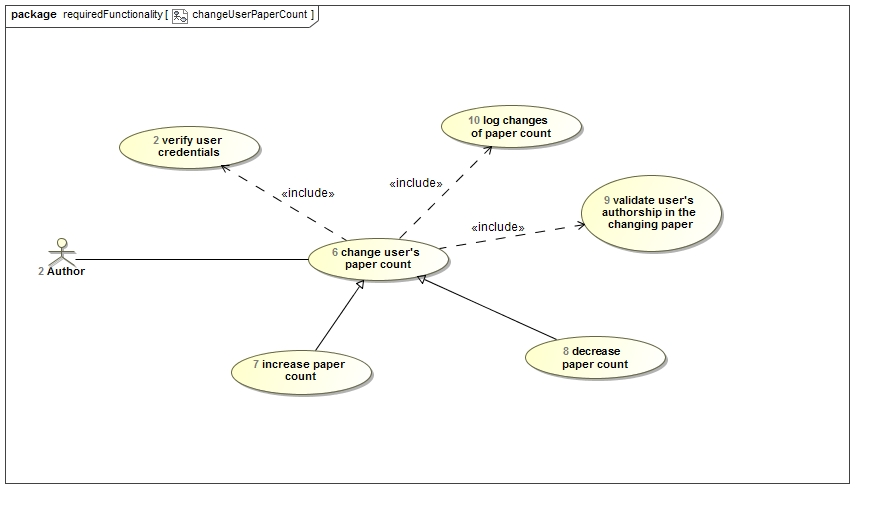
\includegraphics[scale=0.5]{./images/uc__changeUserPaperCount.jpg} 
	\begin{center}
		User profiles should show the total accumulated units
	\end{center}

	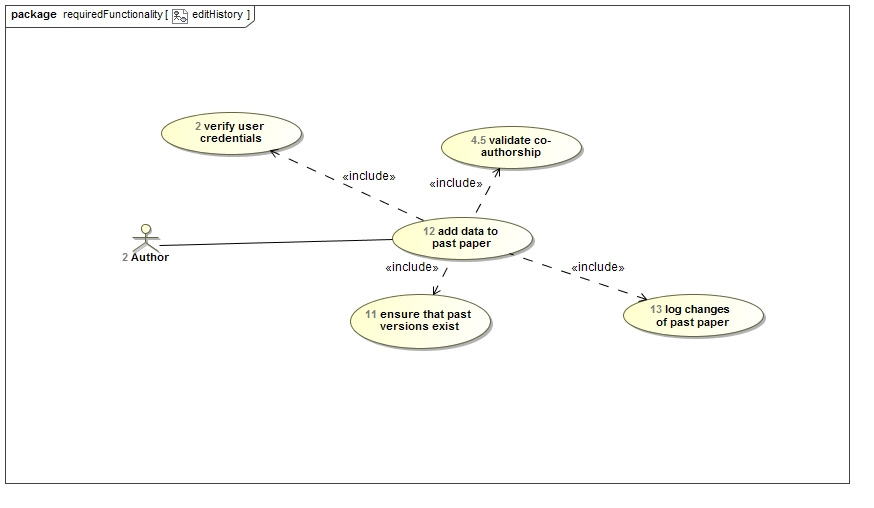
\includegraphics[scale=0.5]{./images/uc__editHistory.jpg}
	\begin{center}
		Users must be able to enter historical data
	\end{center}
\end{flushleft}

\newpage

\begin{flushleft}
	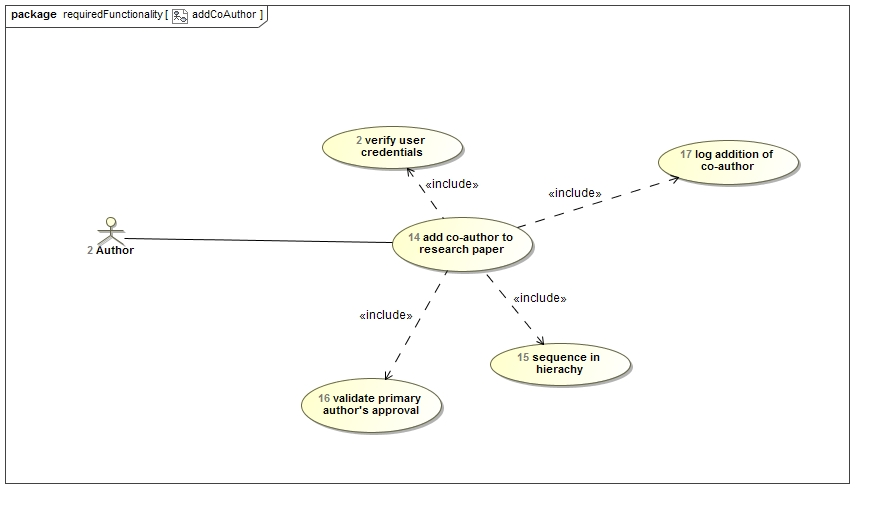
\includegraphics[scale=0.5]{./images/uc__addCoAuthor.jpg} 
	\begin{center}
		Co-authors are added and sequenced
	\end{center}
\end{flushleft}

\subsubsection{Nice-to-have use cases}

\begin{flushleft}
	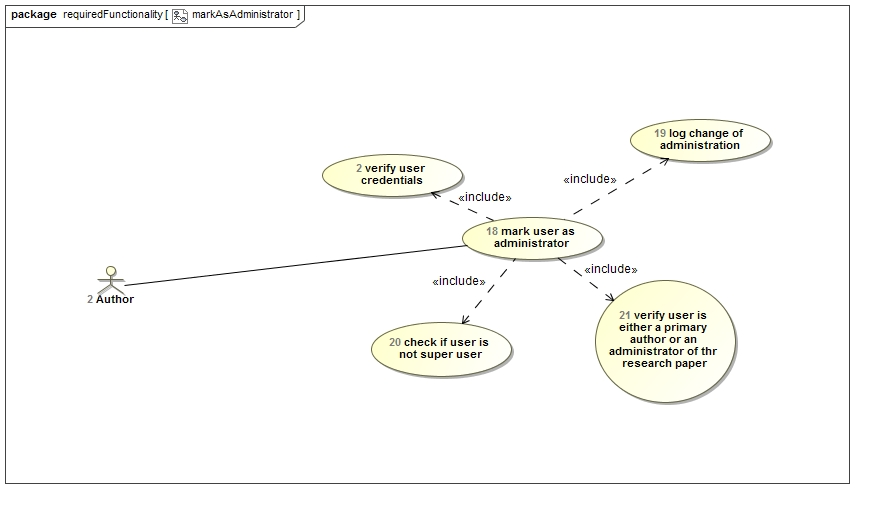
\includegraphics[scale=0.5]{./images/uc__markAsAdministrator.jpg}
	\begin{center}
		Users can be marked as administrators only
	\end{center}

	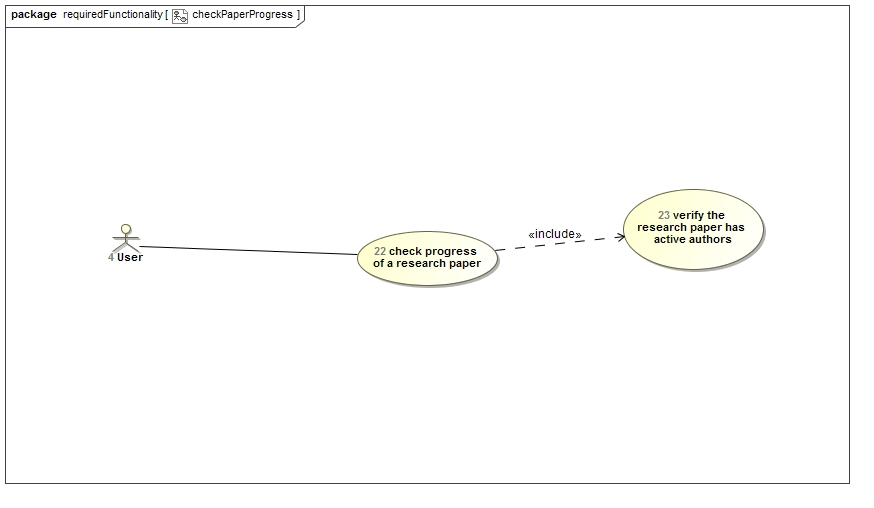
\includegraphics[scale=0.5]{./images/uc__checkPaperProgress.jpg} 
	\begin{center}
		Indication of progress on research project
	\end{center}
\end{flushleft}

\newpage

\begin{flushleft}
	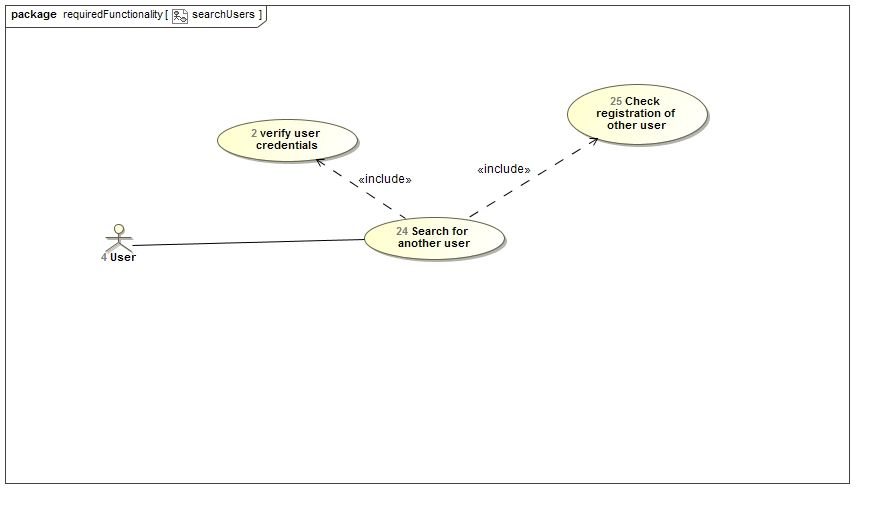
\includegraphics[scale=0.5]{./images/uc__searchUsers.jpg} 
	\begin{center}
		Users should be able to search for other authors
	\end{center}
\end{flushleft}

\subsection{Process specifications}
\subsubsection{Critical use cases}

\begin{flushleft}
	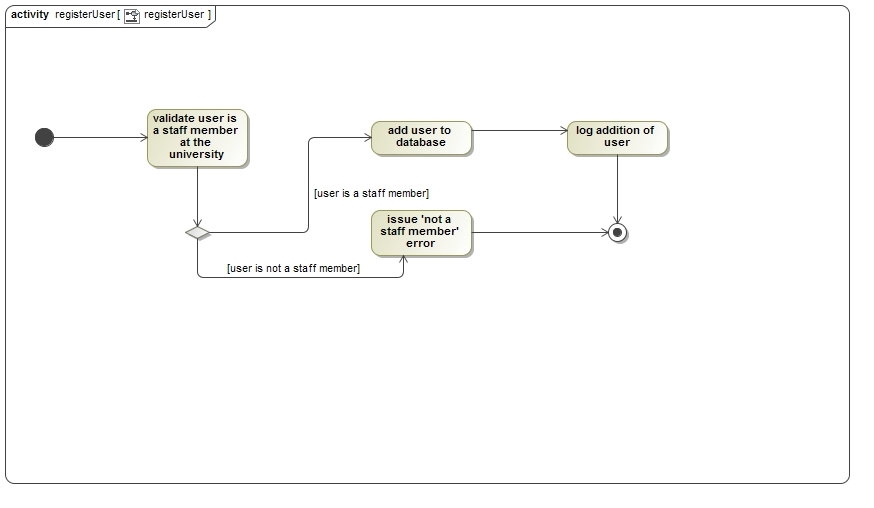
\includegraphics[scale=0.5]{./images/act__registerUser__registerUser.jpg} 
	\begin{center}
		Only UP staff members may register to become users
	\end{center}

	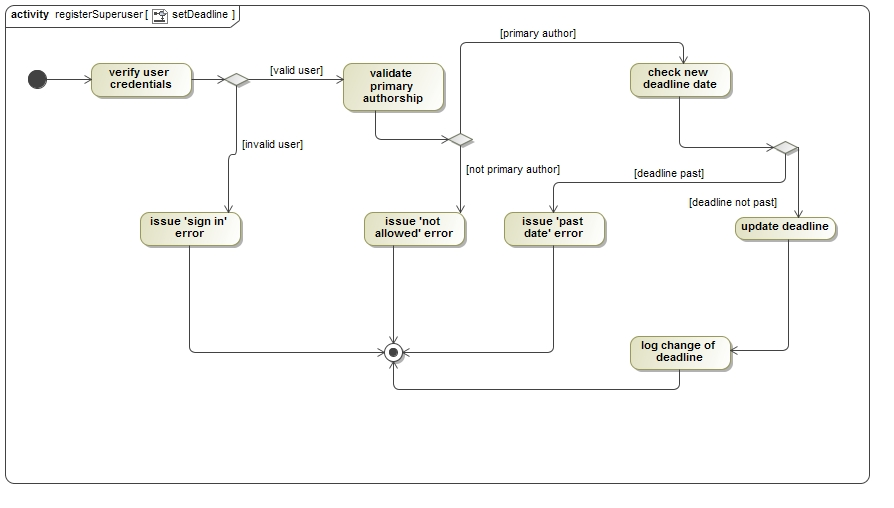
\includegraphics[scale=0.5]{./images/act__registerSuperuser__setDeadline.jpg} 
	\begin{center}
		Creating the super user account
	\end{center}
\end{flushleft}

\newpage

\begin{flushleft}
	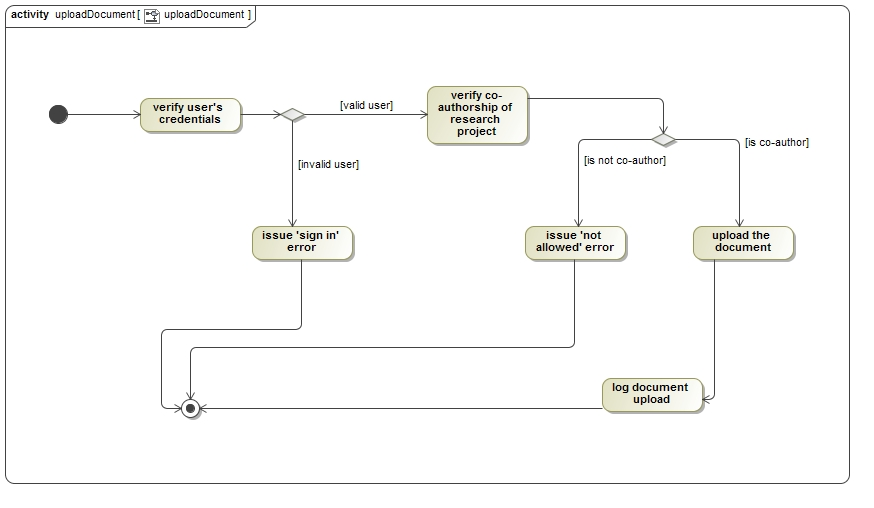
\includegraphics[scale=0.5]{./images/act__uploadDocument.jpg} 
	\begin{center}
		Users should be able to upload their documents
	\end{center}
\end{flushleft}

\subsubsection{Important use cases}

\begin{flushleft}
	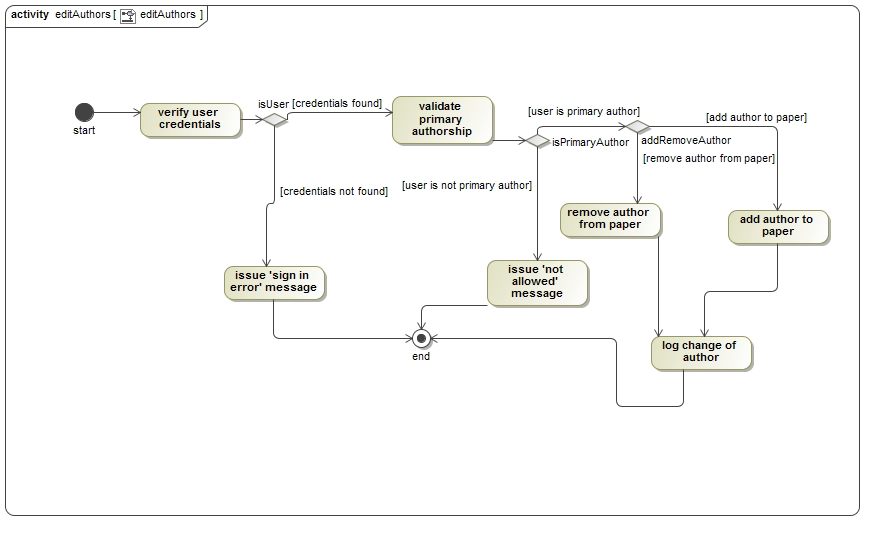
\includegraphics[scale=0.5]{./images/act__editAuthors__editAuthors.jpg} 
	\begin{center}
		Users can add and remove authors
	\end{center}

	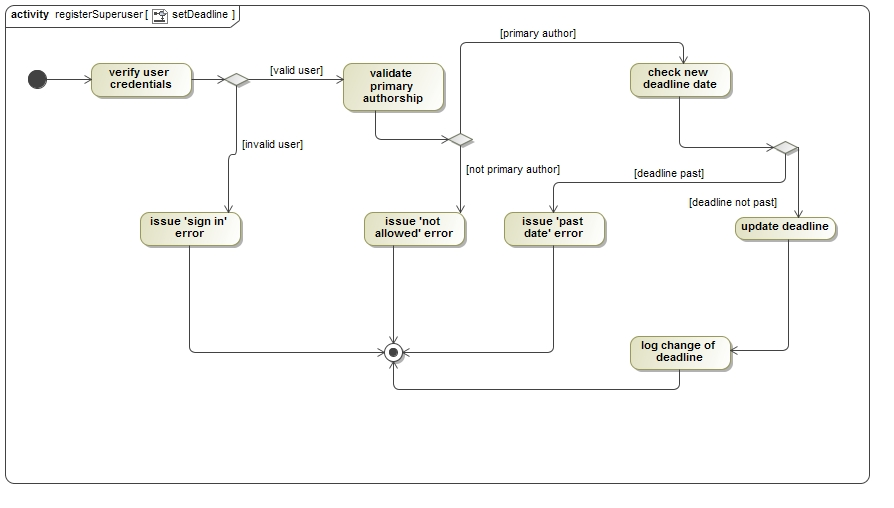
\includegraphics[scale=0.5]{./images/setDeadline.jpg} 
	\begin{center}
		Users decide the deadline of a research project
	\end{center}
\end{flushleft}

\newpage

\begin{flushleft}
	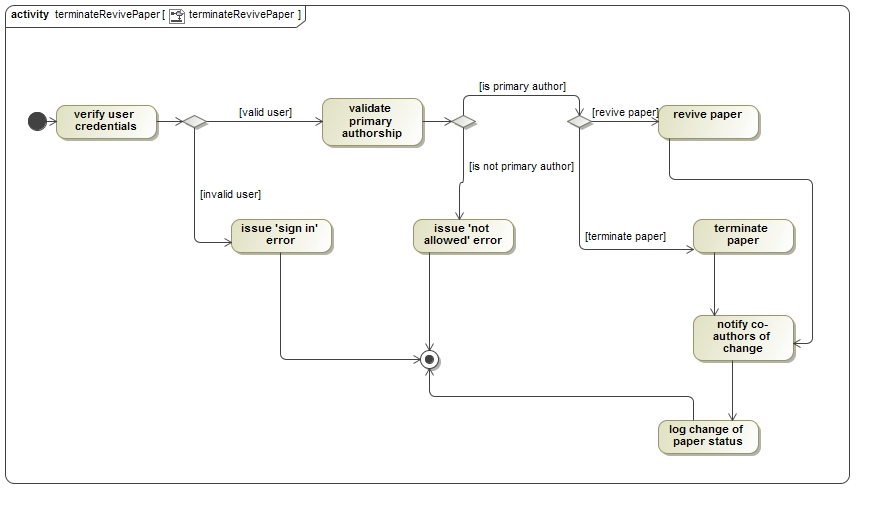
\includegraphics[scale=0.5]{./images/act__terminateRevivePaper__terminateRevivePaper.jpg} 
	\begin{center}
		Users can terminate and revive a research project
	\end{center}

	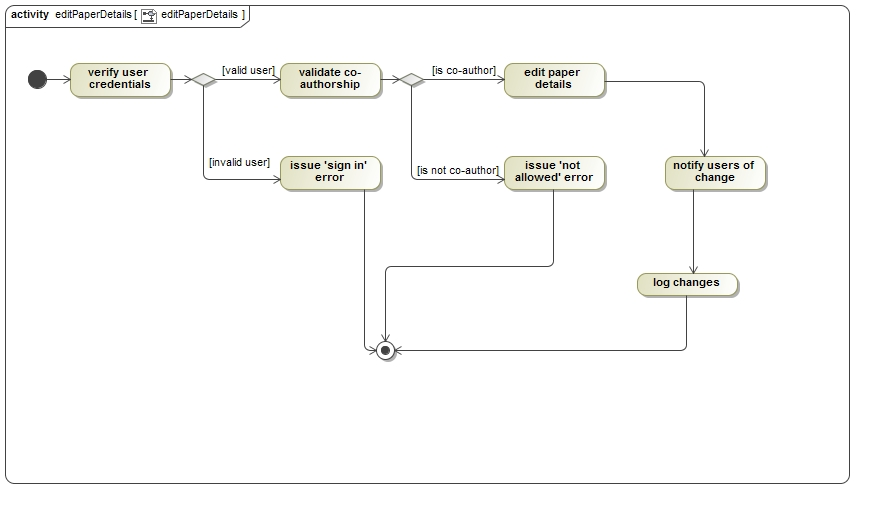
\includegraphics[scale=0.5]{./images/act__editPaperDetails__editPaperDetails.jpg} 
	\begin{center}
		Users can edit details about a research paper they are involved in
	\end{center}
\end{flushleft}

\newpage

\begin{flushleft}
	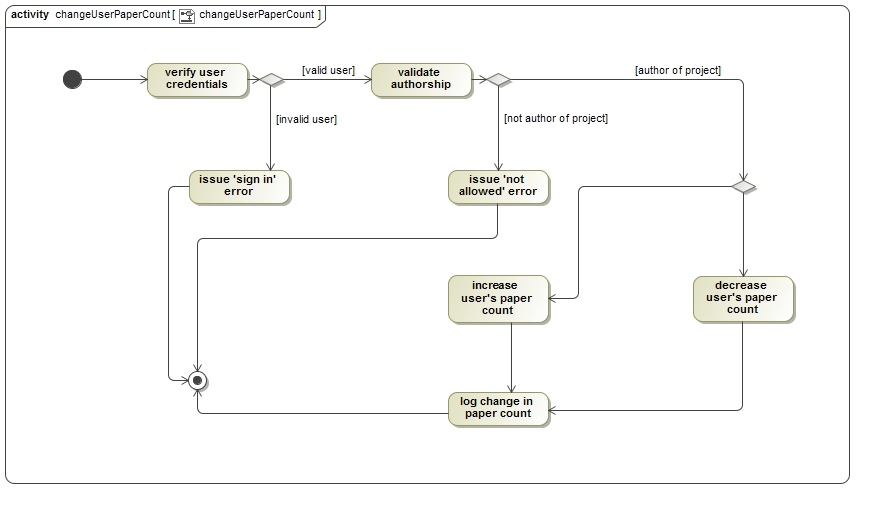
\includegraphics[scale=0.5]{./images/act__changeUserPaperCount__changeUserPaperCount.jpg} 
	\begin{center}
		User profiles should show the total accumulated units
	\end{center}

	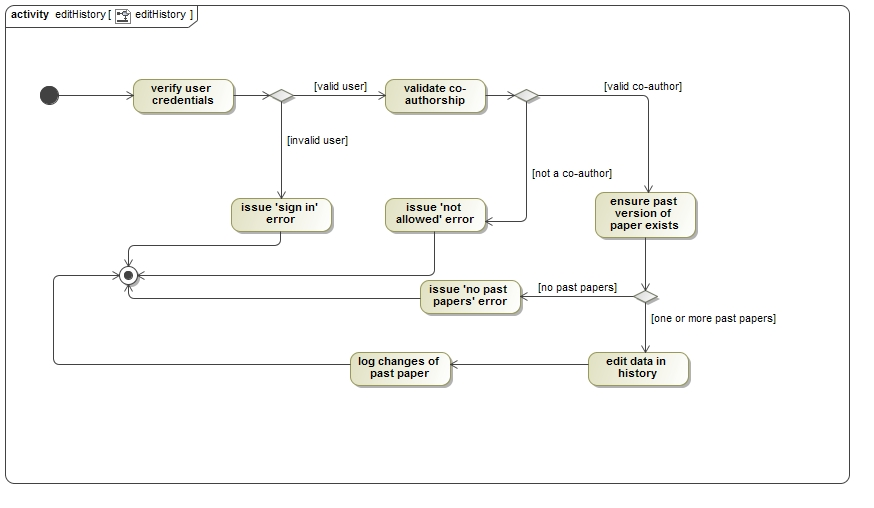
\includegraphics[scale=0.5]{./images/act__editHistory__editHistory.jpg} 
	\begin{center}
		Users must be able to enter historical data
	\end{center}
\end{flushleft}

\newpage

\begin{flushleft}
	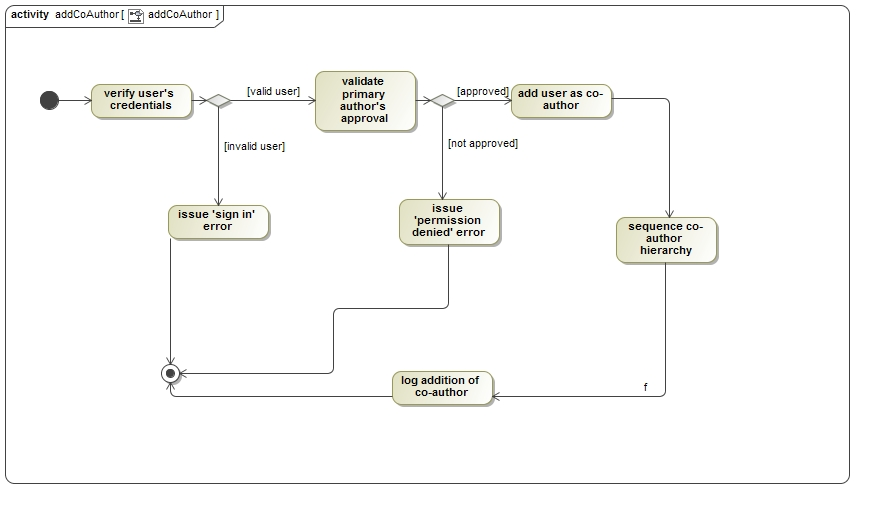
\includegraphics[scale=0.5]{./images/act__addCoAuthor__addCoAuthor.jpg}  
	\begin{center}
		Co-authors are added and sequenced
	\end{center}
\end{flushleft}

\subsubsection{Nice-to-have use cases}

\begin{flushleft}
	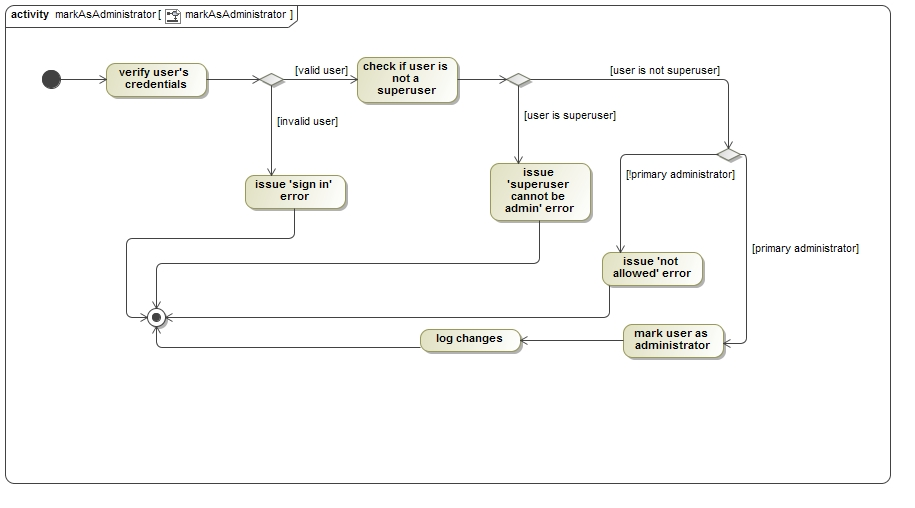
\includegraphics[scale=0.5]{./images/act__markAsAdministrator__markAsAdministrator.jpg} 
	\begin{center}
		Users can be marked as administrators only
	\end{center}

	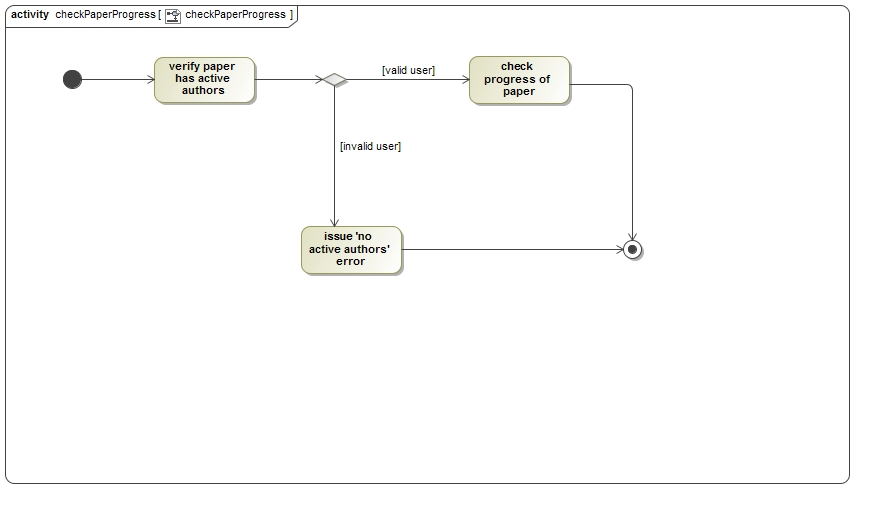
\includegraphics[scale=0.5]{./images/act__checkPaperProgress__checkPaperProgress.jpg} 
	\begin{center}
		Indication of progress on research project
	\end{center}
\end{flushleft}

\newpage

\begin{flushleft}
	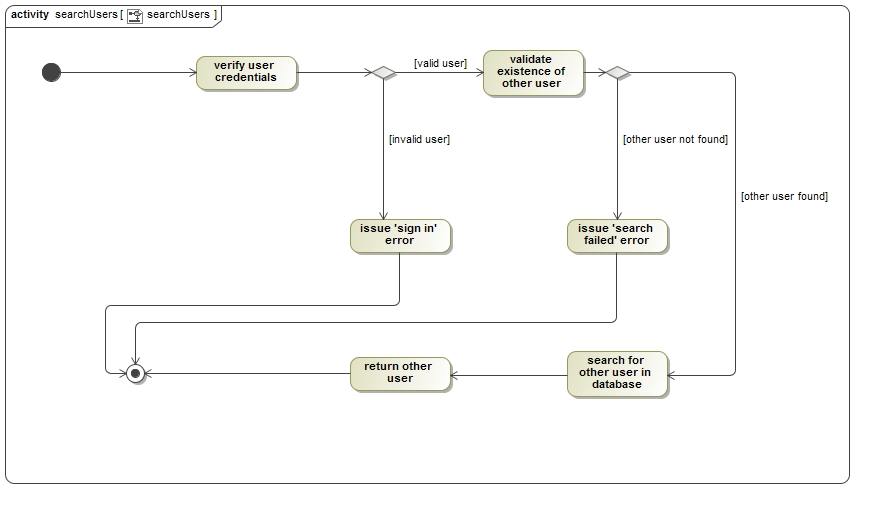
\includegraphics[scale=0.5]{./images/act__searchUsers__searchUsers.jpg} 
	\begin{center}
		Users should be able to search for other authors
	\end{center}
\end{flushleft}

\newpage

\section{Open Issues}
\begin{itemize}
	\item It was never specified whether researchers(non-users) would be able to see the information about the publications they were involved in
	\item Still unclear whether researchers(both users and non-users) will be notified if they are removed from a research group
	\item We are not sure if a user can have multiple sessions open concurrently - if a user is already logged in on the web application, will they be able to log in using their mobile device?
	\item Will the progress be represented by a percentage / a progress bar?
	\item Does the user set the order of the authors or is it automatically set when the user inputs these into a specific document

	\item Is there an option that will be provided for how long before a deadline the user will want to receive a notification?
	\item Won't privacy be an issue if researcher(non-user) information is put up and every user - even those not in the same research group - is able to view it?
	\item Will there be different tabs for different types of publications a user is busy with? ie. screens they can switch between to check on articles, Case reports, terminated publications, etc
	\item Will there be a way that research group members can access each other's information so that they can make contact?
	\item What other applications or platforms must this system be able to integrate with?
\end{itemize}

\end{document}